\documentclass{COMPXXXX}
\usepackage{times}
\usepackage{graphicx}
\usepackage{latexsym}
\usepackage{amssymb}
\usepackage{listings}
\usepackage{lipsum}

\usepackage{latexsym}
\usepackage{amssymb}
\usepackage{algorithm,algpseudocode}
\usepackage{amsmath}
\usepackage{hyperref}
\usepackage{amsthm}


\begin{document}

\title
{GUI Based Network Distributed System for a group-based client-server communication}

\author
{Aziret Asanov\institute{School of Computing and Mathematical Sciences, University of Greenwich, London SE10 9LS, UK, email: aa7726z@gre.ac.uk},~
Tristan P Read\institute{School of Computing and Mathematical Sciences, University of Greenwich, London SE10 9LS, UK, email: tr9529u@gre.ac.uk},~
Kanat Asanov\institute{School of Computing and Mathematical Sciences, University of Greenwich, London SE10 9LS, UK, email: ka8590g@gre.ac.uk}\\
\hspace
    COMP 1549 Advanced Programming\\
	University of Greenwich\\
Old Royal Naval College\\
United Kingdom
        }

\maketitle
\bibliographystyle{COMPXXXX}

\begin{abstract}

\normalsize \textrm {The aim of this coursework is the implementation of a graphical-user interface (GUI), or command-line interface (CLI) based on network distributed system for a group-based client-server communication application which requires research and knowledge of using sockets in Java and its in-built libraries, which include the understanding and implementation of modularity using design patterns, JUnit tests, fault tolerance and component-based development. Which are imperative in the final implementation of the chat-app. In this project we have managed to successfully build and design the server-based chat application within Java.}\\
\textbf{Keywords}\\
\normalsize \textrm {Java, JUnit, Sockets, Graphical-User Interface, Command-Line Interface, Chat-App, Group-Based, Server-based.}

\end{abstract}


\section{I. Introduction}

\normalsize \textrm {The main objective in our coursework is to produce a chat application using the Java programming language and to implement features such as connection, sending private and normal messages between the clients and the host and finally to automate the host’s change if they get disconnected from the server. We have chosen to use GUI due the ease of implementation of private messages and because of the difficulty of handling command line buffers that come with CLI. In our scenario, the main goals of this project were to be able to pass a servers IP, port, and usernames as command-line arguments. To be able to send messages to everyone, between the clients(private messages), to automatically switch hosts if the original had disconnected and to leave notifications to show a message has been received by the specific user. Within this report we aim provide as much information as possible, including the technical sides such as the front end and the back end that was implemented, also the design patterns that were used and JUnit tests to make sure the code is errorless. Chat applications are in the forefront of our lives ranging from WhatsApp, Discord and Telegram and many more thus, why this project is very important in understanding how they work and why Java is the perfect programming language to make these applications.}

\section{II. Design/implementation}

\normalsize \textrm {The development of the code was primarily done using Visual Studio Code which is an integrated development platform that accepts the Java programming language using extensions/plugins and because of its user-friendly experience and features for code debugging and more.\\
We will demonstrate some examples of the design patterns that we have used within this project. The core code of the project that handles networking  consists of four files, two of them handle the server-side logic whilst one of them handles the client-side and the last is a combination of virtual and abstract class where the server and the client extend. The main reasons for choosing this abstract approach were to reduce the amount of duplication within the code, that is because the host and the client sockets in java work in a similar way. Thus, having more flexibility so we can write the same base code for both classes and extend or override the methods as needed.\\
We have considered in making the ChatManager class a singleton class, as only one instance of this class per use is created during testing. However, we have decided to not go forth with this as it makes unit testing easier and allows multiple peers to run under the same process. There are a few times when we make use of the protected variation such as the ServerPeer class which is basically an extension of the peer class, and it also exposes some variables of the main Peer class that should only be modified by the server instance.\\
Another design pattern we have used is the factory pattern, which is used twice within the code, during the creation of the “ServerClientHost” class which is responsible for handling a single connector to another peer and the other is the for the UI Parser. We also use many decorator patterns, particularly in the User-Interface builder which can be found in the “ConfigurationUI.java”.\\
These decorators are used to tell the UI builder to how build certain parts of the UI or how to handle certain events if they do occur. For e.g., if we look at line 93 below in figure 1, we can see that there is an attribute called EventCallbackAttribute, which is attached to the method called Connect Click and the use of this decorator tells the UI builder that when the “Connect button” is clicked, it should call the method “Connect Click".}\\
\begin{figure}
\centering
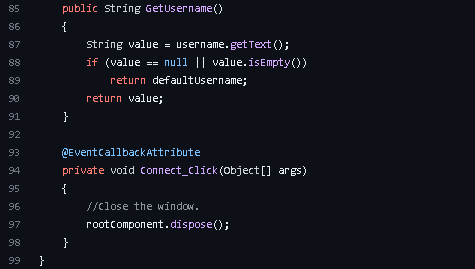
\includegraphics[width=1.0\linewidth]{Connect Click.png}
\caption{}
\label{fig:figure01}
\end{figure}

\normalsize \textrm {Now, about modularity and component design side of the code. When writing programs its best to try and make them as modular as possible, meaning that no one part of the program is packed too tightly together. This enables reusability of the code to be used within the project and within other future projects. This program has been split into two main packages, the first is the ‘readiefur’ package which contains all the modular code that is not specific to this project alone for reusability. The second is the chat-app package which contains all the codes specifically for this project. Having a look at some of the files within the ‘readiefur’ package for example, the file ‘XMLUI.java’ is seen that only the java built-in libraries and those specific to the readiefur.xml-ui packages are being used, showing that this file is not dependent on any other files used within the project, meaning we can reuse the code elsewhere.\\
A good example of a component used within this project out of many is the “ServerClientHost.java class which is responsible for handling a single connection to another peer(client). This component is made in a way where it is capable of being created multiple times due to the expectation that many peers(clients) want to connect to the same server and this in return handles that foreseen scenario and enables multitude of connections to be made and this is where the component “ServerClientHost.java” is used for.}\\
\begin{figure}
\centering
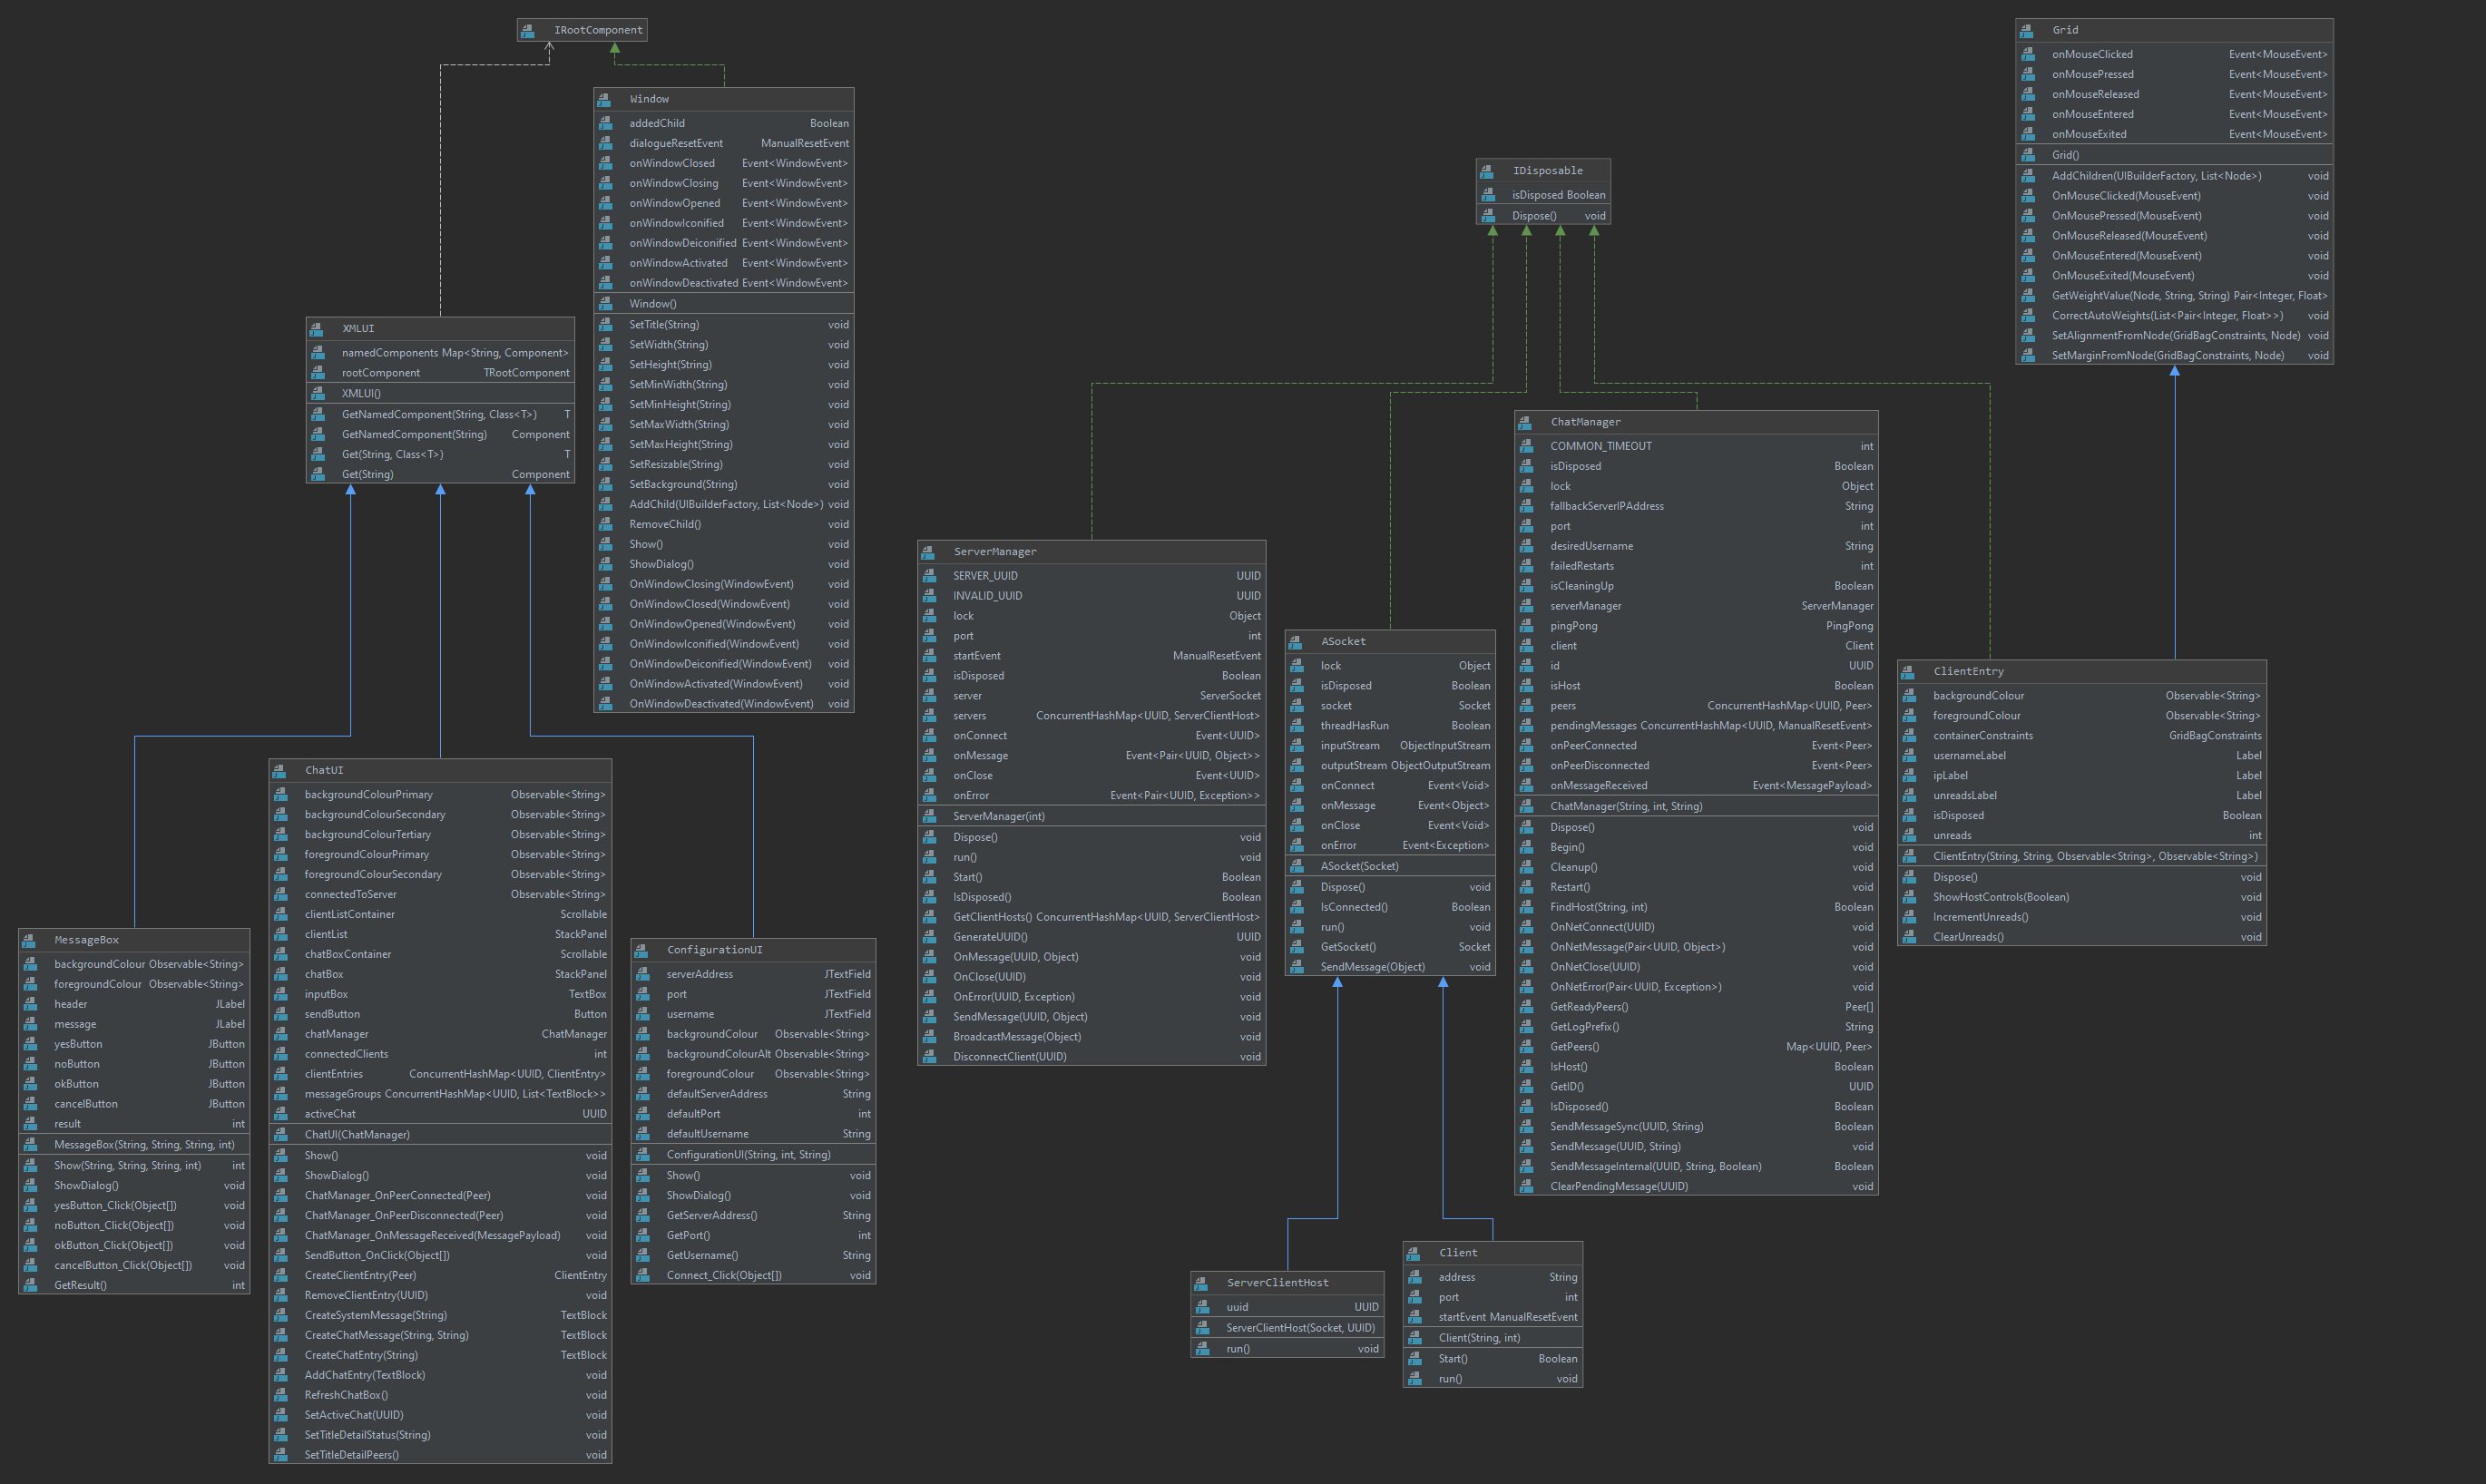
\includegraphics[width=1.0\linewidth]{All UML.png}
\caption{UML Diagram for all classes}
\label{fig:figure02}
\end{figure}

\section{III. Analysis and Critical Discussion}
\normalsize \textrm {Unit testing is important with projects as big as these as they require you to debug and find errors within the code. In our case, we were originally going to run unit tests on the front-end UI only to realise that there were no elements appearing on the UI tree and with research it was found that Java  Swing framework does not comply with the Windows Accessibility API that we have used for the project because Java uses its own rendering engine. Thus, why we couldn’t do automated front-end unit tests. Involving the backend unit tests on the other hand worked, so we have made unit tests on ChatManager class which can be found in the src/testing/Backend.java. where the test is used to check that one instance becomes the host and the other becomes the client. This can be found below in figure 3}\\
\begin{figure}
\centering
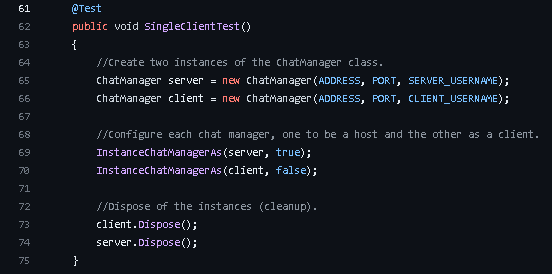
\includegraphics[width=1.0\linewidth]{Unit Test on ChatManager.png}
\caption{}
\label{fig:figure03}
\end{figure}

\normalsize \textrm {A more complex test which was written is one that will check if a private message is received by the correct peer(client). This test will create three instances of the ChatManager class, one will be the host and the other two will be clients. The test will then send a private message from a peer to another peer, and it will check that only the target peer received the private message.}

\normalsize \textrm {In this first image "figure 4" we can see a message being broadcasted to all clients.\\
\begin{figure}
\centering
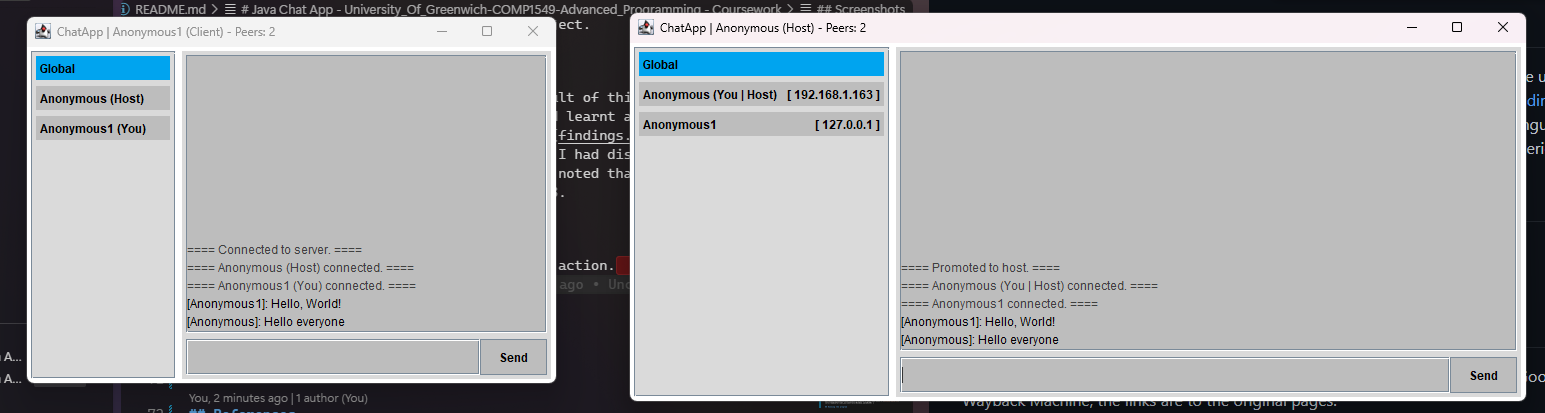
\includegraphics[width=1.0\linewidth]{broadcast_message.png}
\caption{}
\label{fig:figure04}
\end{figure}\\
In this next image "figure 5" we can see that the server has sent a private message to a client, and the client has received a notification indicating that they have an unread message.\\
\begin{figure}
\centering
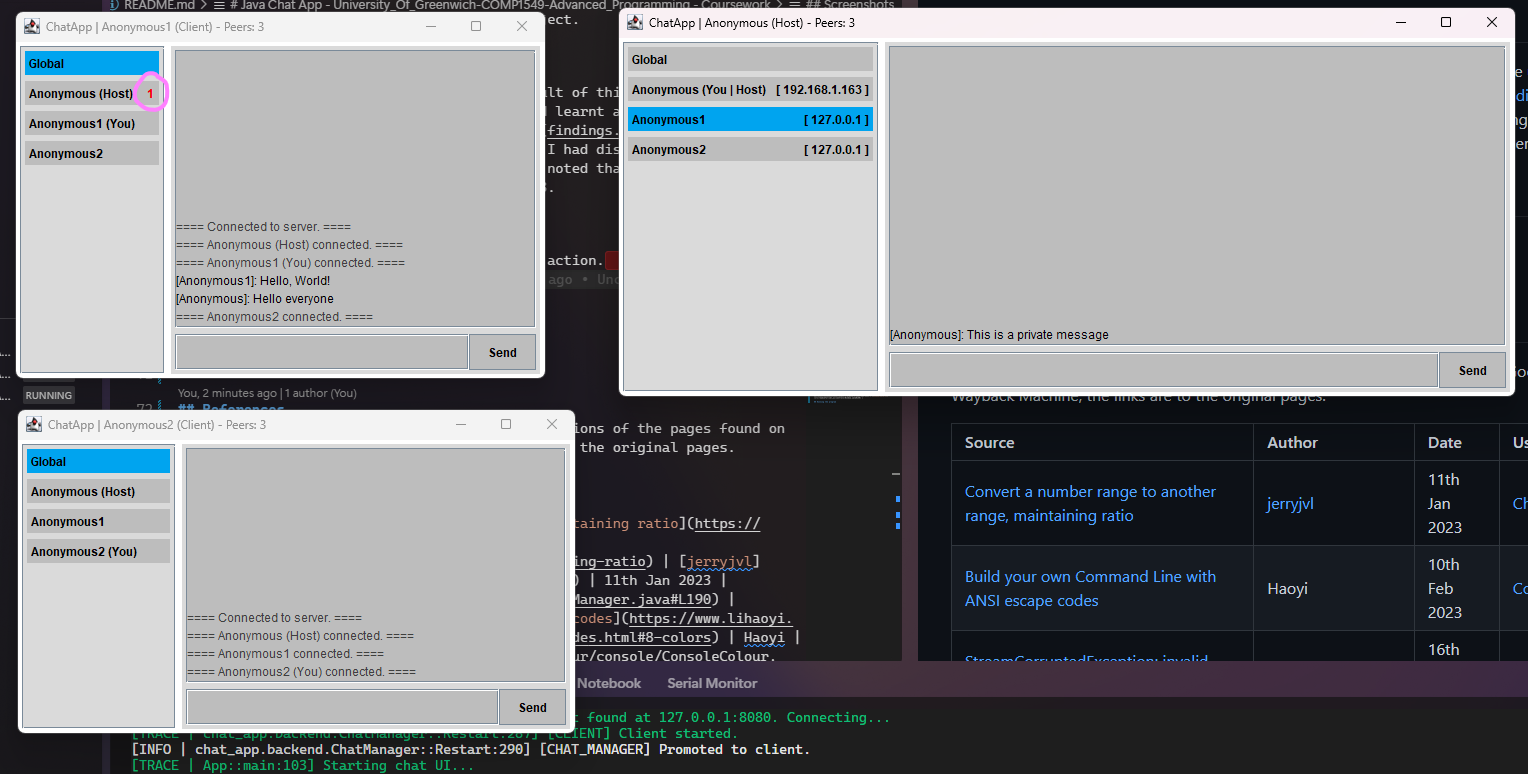
\includegraphics[width=1.0\linewidth]{unread_message 2.png}
\caption{}
\label{fig:figure05}
\end{figure}\\
In this image "figure 6" we can see that the peer "Anonymous1" has received a private message from the peer "Anonymous" and that the peer "Anonymous2" cannot see the message.\\
\begin{figure}
\centering
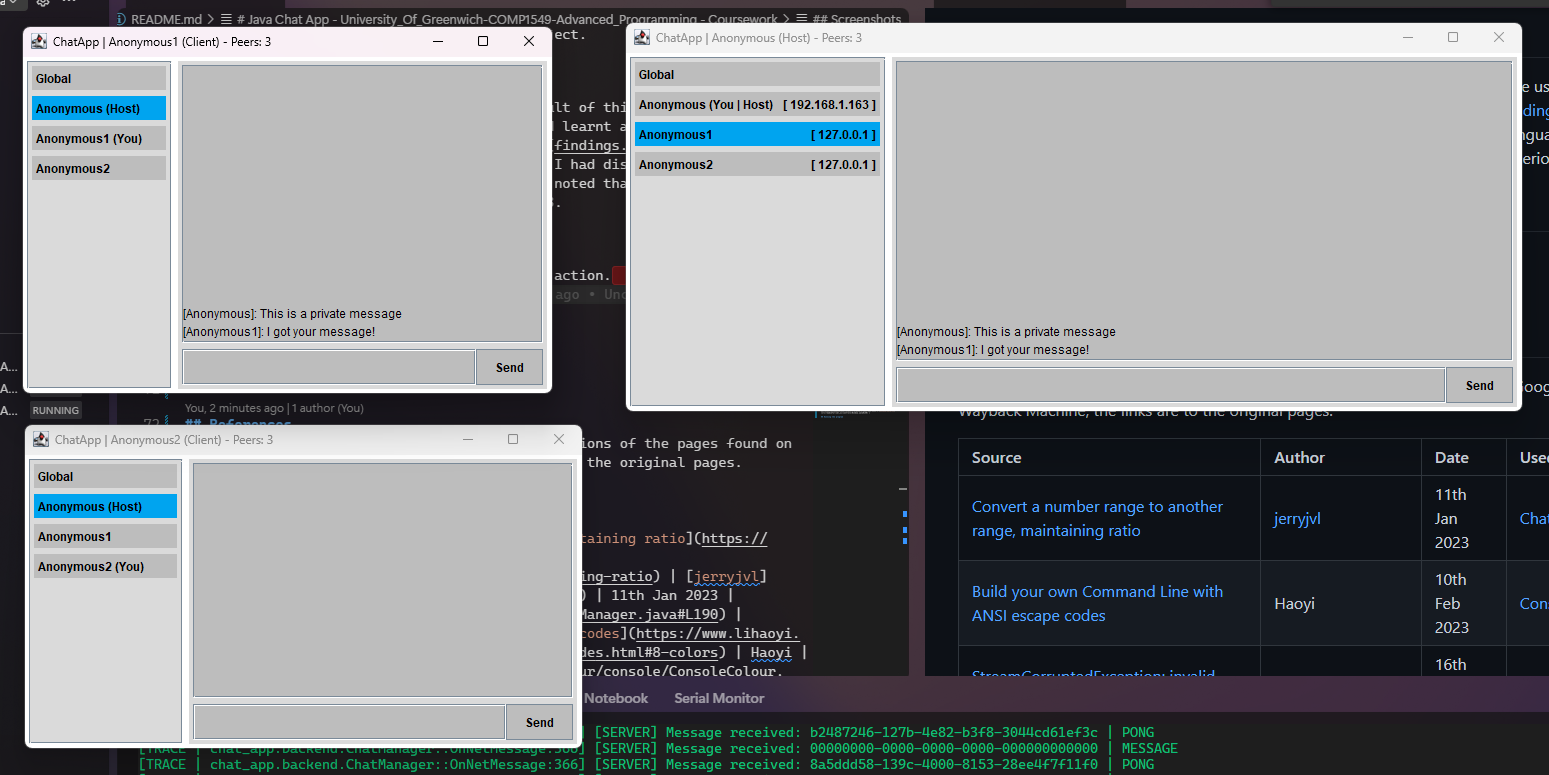
\includegraphics[width=1.0\linewidth]{private_message 3.png}
\caption{}
\label{fig:figure06}
\end{figure}\\
In this image "figure 7" we can see that a system message has been placed into the global chat, indicated by a prefix and suffix of ==== as well as being in a light grey colour, that the peer "Anonymous1" has disconnected.\\
\begin{figure}
\centering
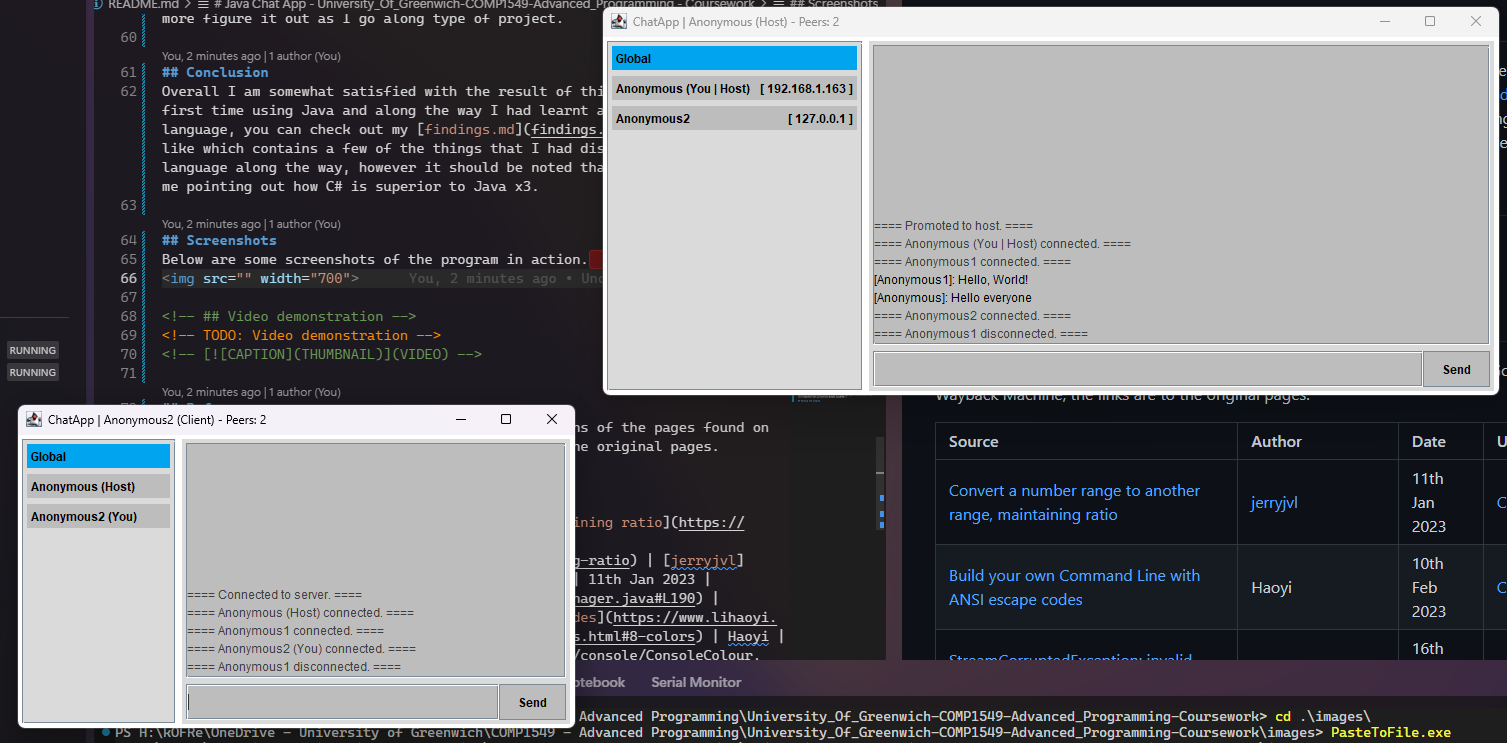
\includegraphics[width=1.0\linewidth]{client_disconnect 4.png}
\caption{}
\label{fig:figure07}
\end{figure}\\
In this final image "figure 8" we can see that the server has disconnected and that one of old clients have become the server and the other old client has automatically connected to the new server.\\
\begin{figure}
\centering
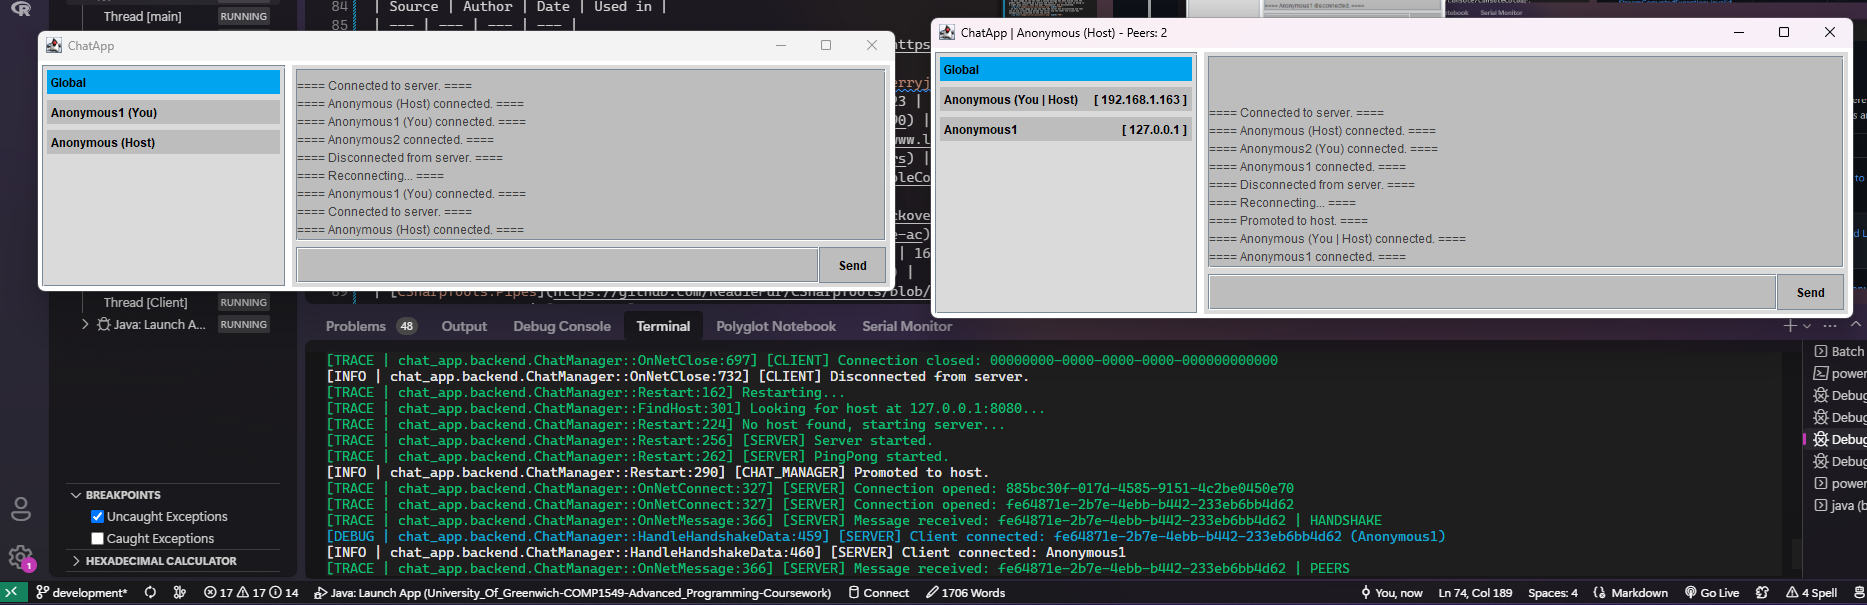
\includegraphics[width=1.0\linewidth]{server_disconnect 5.png}
\caption{}
\label{fig:figure08}
\end{figure}}


\normalsize \textrm {Also, some additional features include the readiefur.xml-ui package which is a simplified framework of the in-built Java Swing UI as it seemed too repetitive in the code. We also made it so that the UI building starts within the XMLUI class, where all the custom elements will extend from this virtual class and specify the root component types as the generic parameters. Then using reflection, the virtual class will search for an xml file with the same class name as the one that extends it. Also, a log manager which is basically an extra debugging tool.\\
The next file is the UIBuilderFactory class. In this class is where the XML file is parsed into a tree of Java Swing component objects. Inside of it is a recursive method called “ParseXMLNode” which is the first stage in converting the XML node into a Java Swing Component object. This method applies common properties such as the name of the element, also configuring any binding attributes, as well as applying any custom properties that it finds on the corresponding Java class for that XML node. Then the method will call the ParseChildTree on the component wrapper, which will then compute any other properties for that given element and recursively call the ParseXMLNode method on each child node if applicable. Once that is finished the root Java Swing Component object will have returned and set as rootComponent variable of the XMLUI class, which the extended class can call upon.\\
Bugs & Exception Handling
In our code we had used exception handling such as try and catch to find bugs early on within the code and throughout.\\
While we have tried to keep the program as bug free as possible, it is almost always inevitable that bugs will be present in any program.\\
For the most part, in the manual testing we have experienced very few bugs, however there is one that has been noticed that had no easy fix.\\
Unfortunately, this bug is extremely difficult to reproduce, therefore making it equally as hard to fix. The bug will occur at startup when a client is trying to connect to a server. We are unsure as to what exactly is causing this issue; however, we think it could be a race condition on our automatic migration system, this could also explain why the bug is so hard to reproduce. But then looking at the error log and stack trace, the error seems to lie in parsing the data received which after reading the error code online, is due to corrupt data. This bug is a fatal bug to our project because it renders the entire application unusable and floods the console with this error indefinitely. Below you can see a screenshot of the error and the stack trace.\\
Picture of the bug is in figure 9.\\
\begin{figure}
\centering
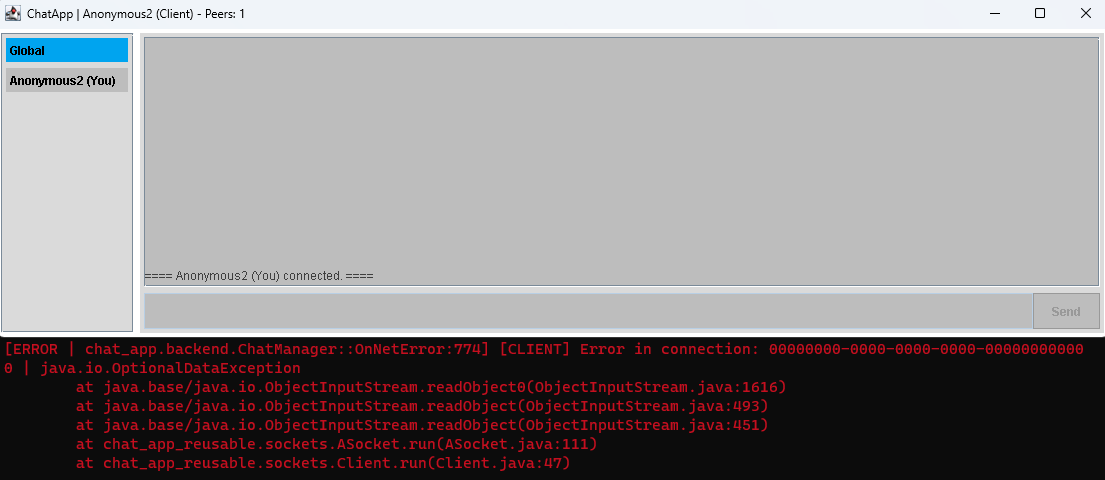
\includegraphics[width=1.0\linewidth]{Bug.png}
\caption{}
\label{fig:figure09}
\end{figure}}

\section{IV. Conclusion}

\normalsize \textrm {Overall, the coursework was deemed a success as that bug only occurs rarely, we have enjoyed this coursework and we have managed to create  a chat-app that had made use of many components and UI libraries. In conclusion, this project was complex and required fine skills, on the other hand, was enjoyable as it was very engaging. This is also due to the fact that as a group we were capable of sharing our knowledge and expertise within certain areas. Overall, we managed to successfully design, create and run the Graphical User Interface (GUI) based networked distributed system for a group-based client-server communication. This includes all the specified requirements set out from the beginning of the project. This chat based application shows its practicality and value, as it allows the users to communicate with each other, on a functional and secure system, whereby a user-friendly graphical user interface makes it more untroublesome to utilise and operate.}

\ack

\normalsize \textrm {We can write this some other day together.}

\normalsize \textrm {}

\section{References}

\normalsize \textrm {Author: jerryjvl\\
https://stackoverflow.com/questions/929103/convert-a-number-range-to-another-range-maintaining-ratio\\
Used in: ChatManager.java:190\\
Date used: 11th Jan 2023\\
Author: Haoyi\\
https://www.lihaoyi.com/post/BuildyourownCommandLinewithANSIescapecodes.html\\
Used in: ConsoleColour.java\\
Date used: 10th Feb 2023\\
Author: user207421\\
https://stackoverflow.com/questions/2393179/streamcorruptedexception-invalid-type-code-ac\\
Used in: ASocket.java:20\\
Date used: 16th Feb 2023\\
Author: ReadieFur / Tristan Read\\
https://github.com/ReadieFur/CSharpTools/tree/main/src/CSharpTools.Pipes\\
Used in: ServerManager.java\\
Date used: 27th Jan 2023\\
Author: Oracle\\
https://docs.oracle.com/javase/7/docs/api/java/awt/event/WindowListener.html\\
Used in: Window.java:40\\
Date used: 31st Jan 2023}

\end{document}
